\documentclass{article}
\usepackage[T1]{fontenc}
\usepackage{lmodern}
\usepackage[polish]{babel}
\usepackage{graphicx}
\usepackage{float}
\usepackage{hyperref}
\usepackage{amsmath} 
\usepackage{multicol}
\usepackage{listings}
\usepackage{tikz} % pgf package
\usetikzlibrary{shapes.multipart}
\usepackage[shortlabels]{enumitem}
\usepackage{fancyhdr}

\usepackage[justification=centering]{caption}

\usepackage[a4paper, margin=2.54cm]{geometry}

\pagestyle{fancy}
\fancyhf{}
\fancyhead[L]{\leftmark}
\fancyfoot[C]{\thepage}
\setlength{\headheight}{13pt}
\addtolength{\topmargin}{-1pt}

\lstdefinestyle{siec}{
    basicstyle=\ttfamily\footnotesize,
    frame = tb,
    title={Struktura sieci},
    backgroundcolor=\color{gray!10},
}

\title{Sprawozdanie z projektu ze Sztucznej Inteligencji \\ 
Porównanie metod uczenia maszynowego \\ 
w problemie MNIST i jego pochodnych}
\author{Filip Gołaś s188776 \\ Damian Jankowski s188597 \\ Mikołaj Storoniak s188806}

\begin{document}

\maketitle

\begin{multicols}{2}
    \tableofcontents
\end{multicols}

\newpage

\section{Opis problemu}

Celem projektu było zbudowanie i porównanie różnych
modeli uczenia maszynowego w problemie klasyfikacji
obrazów z bazy MNIST. Korzystaliśmy głównie z bazy
danych \textbf{MNIST-784}, która zawiera 70 tysięcy obrazów
cyfr napisanych ręcznie. Każdy obraz jest w skali
szarości i ma rozmiar 28x28 pikseli. Każdy piksel
jest reprezentowany przez liczbę całkowitą z zakresu
od 0 do 255, która określa jasność piksela. Dodatkowo
każdy obraz ma przypisaną etykietę, która określa
jaką cyfrę przedstawia obraz.

\begin{figure}[H]
    \centering
    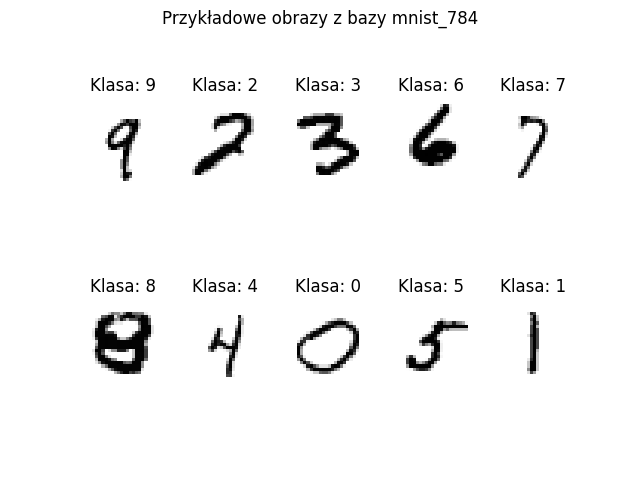
\includegraphics[width=0.8\textwidth]{img/baza_mnist_784.png}
\end{figure}

Zdecydowaliśmy się również na wykorzystanie bazy
danych \textbf{Fashion-MNIST}, która podobnie jak poprzednia, zawiera
70 tysięcy obrazów o rozmiarze 28x28 pikseli, natomiast
każdy obraz przedstawia wybrane ubranie lub akcesorium.

\begin{figure}[H]
    \centering
    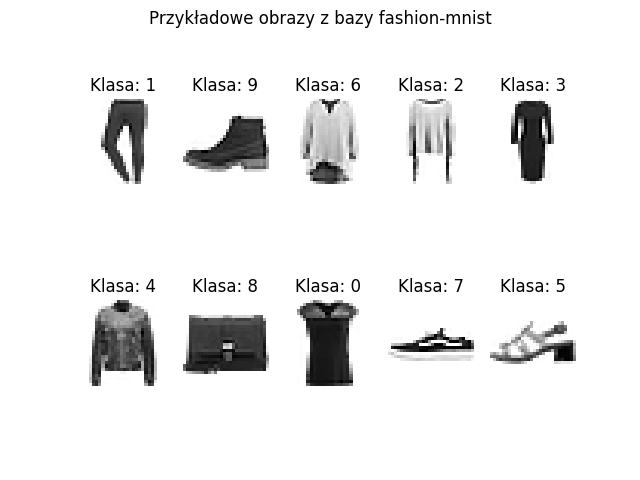
\includegraphics[width=0.8\textwidth]{img/baza_fashion_mnist.png}
\end{figure}

Opis klas w bazie danych Fashion-MNIST:

\begin{enumerate}
    \begin{multicols}{2}
        \centering
        \setcounter{enumi}{-1}
        \item T-shirt/top
        \item Trouser
        \item Pullover
        \item Dress
        \item Coat
        \item Sandal
        \item Shirt
        \item Sneaker
        \item Bag
        \item Ankle boot
    \end{multicols}
\end{enumerate}

\section{Opis aplikacji}
W ramach projektu stworzono aplikację służącą do testowania różnych modeli nauczania maszynowego dla
problemu MNIST i jego pochodnych. Aplikacja umożliwia pobranie
dowolnej bazy danych problemu klasyfikacji obrazu podobnej
do MNIST ze strony OpenML. Następnie użytkownik może wybrać
jeden z zaimplementowanych modeli, wytrenować go oraz przeprowadzić
szereg testów. Przede wszystkim jednak aplikacja umożliwia
ręczne rysowanie obrazu do klasyfikacji, lub wczytanie i
modyfikację już istniejącego w bazie obrazu.

\begin{figure}[H]
    \centering
    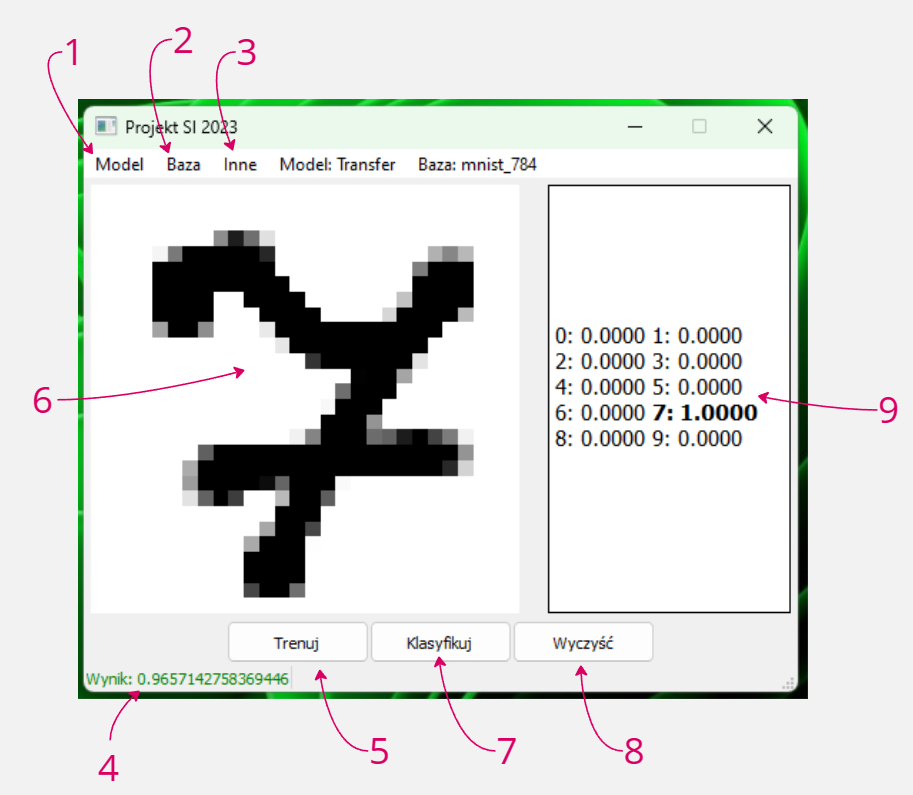
\includegraphics[width=0.6\textwidth]{img/gui.png}
\end{figure}

\begin{enumerate}
    \item Model - zawiera opcje utworzenia
     nowego modelu spośród zaimplementowanych,
     zapisanie już wytrenowanego modelu oraz wczytanie
     modelu z pliku.
    \item Baza - zawiera opcje pobrania bazy danych
     z serwisu OpenML i wczytania pobranej bazy z pliku.

    \item Inne - zawiera opcje:
        \begin{itemize}
            \item Wczytania losowego obrazu wybranej klasy z załadowanej bazy
            \item Walidacji modelu na zbiorze testowym załadowanej bazy
            \item Kroswalidacji modelu dla wybranej ilości podziałów
            \item Generowanie macierzy konfuzji
            \item Opcję włączenia przetwarzania obrazów tak by były kompatybilne z bazą MNIST-784. W przypadku modyfikowania obrazów wczytanych z bazy lub korzystania z bazy innej niż MNIST-784 należy odznaczyć tę opcję.
            \item Opcję wyświetlania danych wejściowych, które otrzyma model w postaci obrazka
        \end{itemize}

    \item Pasek stanu - wyświetla informacje o stanie aplikacji oraz komunikaty, w tym informacje o błędach i niektóre wyniki walidacji
    \item Trenuj - przeprowadza proces uczenia modelu na załadowanej bazie danych. Gdy jest to możliwe generuje i pokazuje wykresy z przebiegu procesu trenowania
    \item Kanwa - na niej można dokonywać zmian obrazu, który dostanie model do klasyfikacji
    \item Klasyfikuj - wciśnięcie tego przycisku rozpocznie proces walidacji obrazu widocznego na kanwie. Obraz będzie poddany przetwarzaniu, jeżeli ta opcja z menu Inne jest wybrana.
    \item Wyczyść - czyści kanwę
    \item Wyniki klasyfikacji - wyświetla wyniki klasyfikacji obrazu do poszczególnych klas.
\end{enumerate}

Proces przetwarzania obrazów z kanwy jest niezwykle ważny
w przypadku odręcznego rysowania cyfr dla modelu uczonego
na bazie MNIST-784. Obrazy obecne w tej bazie muszą spełniać
pewne założenia, dlatego model nie jest w stanie rozpoznawać
cyfr, które drastycznie róznią się od tych obecnych w bazie.
W celu przetwarzania obrazów z kanwy stosuje się:
\begin{itemize}
    \item Skalowanie - cyfra w bazie mnist musi mieć rozmiar $20\times20$ pikseli mimo, że obrazy w bazie maja rozmiar $28\times28$ pikseli. W tym celu do rozmiaru $20\times20$ pikseli skalowany jest prostokąt zawierający niezerowe piksele obrazu a następnie reszta uzupełniana jest zerami.
    \item Środkowamie - obraz przesuwany jest tak, by jego środek masy znajdował się w środku obrazu $28\times28$ pikseli
\end{itemize}



\section{Opis porównanych modeli}

\subsection{Drzewa}
\subsubsection{Drzewo decyzyjne}
Drzewo decyzyjne jest modelem predykcyjnym wykorzystywanym w 
dziedzinie uczenia maszynowego i analizy danych. Jest to 
struktura drzewiasta, w której każdy węzeł reprezentuje 
test na jednej z cech, gałęzie reprezentują możliwe wyniki 
tego testu, a liście reprezentują etykiety lub wartości 
predykcyjne. Drzewo decyzyjne może być wykorzystane 
zarówno do klasyfikacji, jak i do regresji.

Podczas konstrukcji drzewa decyzyjnego, 
algorytm dokonuje podziału zbioru danych 
na podzbiory na podstawie wybranych cech. 
Celem jest jak najlepsze rozdzielenie danych, 
aby w każdym podzbiorze dominowała jedna klasa 
lub aby zminimalizować błąd predykcji dla zmiennych 
ciągłych w przypadku regresji.

Drzewa decyzyjne posiadają wiele zalet, takich jak 
prostota interpretacji, zdolność do obsługi zarówno 
danych kategorycznych, jak i numerycznych, oraz efektywność 
obliczeniowa w przypadku dużych zbiorów danych. Jednakże, 
mogą być podatne na przetrenowanie, co oznacza, że mogą zbyt 
dobrze dopasować się do danych treningowych i słabo generalizować na nowe dane.

\subsubsection{Las losowy}
Las losowy (ang. Random Forest) jest złożonym modelem 
predykcyjnym, który opiera się na kombinacji wielu drzew decyzyjnych. 
Polega na budowie wielu drzew decyzyjnych na podstawie 
różnych losowych podzbiorów danych treningowych, a 
następnie łączeniu ich wyników w celu uzyskania ostatecznej 
predykcji. Każde drzewo w lesie losowym jest budowane 
niezależnie od pozostałych, a wyniki są łączone w procesie 
głosowania lub uśredniania.

Las losowy ma wiele zalet, w tym wysoką dokładność 
predykcji, zdolność do obsługi zarówno danych 
kategorycznych, jak i numerycznych, oraz odporność 
na przetrenowanie. Dodatkowo, las losowy może dostarczać 
ważność cech, co oznacza, że można ocenić, które cechy 
mają największy wpływ na predykcje.

Las losowy znajduje zastosowanie w wielu dziedzinach, 
takich jak klasyfikacja obrazów, przetwarzanie 
języka naturalnego, analiza danych medycznych itp. 
Jest to popularny model ze względu na swoją elastyczność 
i dobrą wydajność nawet w przypadku dużych zbiorów danych.

\subsection{Sieci neuronowe}
Sieć neuronowa jest modelem statystycznym czerpiącym inspirację z natury i 
działania układów nerwowych żywych organizmów.
Modele te są stosowane zarówno do problemów regresji (aproksymacji) jak i klasyfikacji
poprzez nauczanie nadzorowane.

Podstawową składową każdej sieci neuronowej jest neuron, który może być reprezentowany 
jako funkcja wielu parametrów zwracająca dyskretną wartość
prawda lub fałsz. Choć jeden neuron nie jest w stanie opisać złożonych modeli, 
dużo większe możliwości mają sieci neuronowe zbudowane z wielu neuronów
połączonych w warstwy w taki sposób, że wynik jednej warstwy służy jako parametry kolejnej.

% TU WSTAWIĆ ILUSTRACJĘ WARSTW PRZEKAZUJĄCYCH SOBIE PARAMETRY

Poprzez odpowiednie ustawienie współczynników funkcji w neuronach jesteśmy w 
stanie zamodelować zależności dużo bardziej złożone niż te możliwe do opisania jedną
prostą funkcją wielu parametrów.

\subsubsection{Wielowarstwowy perceptron}

W praktyce w sieciach neuronowych neurony są zastąpione perceptronami, które od neuronów 
różnią się tym, że są funkcjami w dziedzinie rzeczywistej.
Same warstwy neuronów również nie są reprezentowane jako zbiory obiektów typu neuron. 
Operacja przechodzenia danych wejściowych przez kolejne warstwy sieci
zwana propagacją w przód może być zrealizowana w każdej warstwie poprzez proste mnożenie macierzy

\begin {equation}
    S = X \times W
\end{equation}
gdzie:
\begin{itemize}
    \item $X$ jest macierzą $(n, 1)$ parametrów będących danymi 
    wejściowymi sieci w przypadku warstwy pierwszej (wejściowej), 
    lub wartości zwróconych przez poprzednią warstwę w sieci
    \item $W$ jest macierzą $(m, n)$ współczynników funkcji opisujących perceptrony, 
    w której każdy wiersz opisuje jeden perceptron, 
    a każda kolumna odpowiada wartości współczynnika tego perceptronu dla danego parametru 
    z wektora wejściowego warstwy
    \item $S$ jest macierzą wynikową warstwy $(1, m)$ zawierającą wartości zwrócone przez 
    funkcje opisujące perceptrony tworzące tę warstwę
\end{itemize}

Następnie należy zdecydować kiedy uznamy dany neuron za pobudzony. Do tego zadania 
stosuje się funkcje aktywacji, których dobór jest niezwykle ważny
i może łatwo zadecydować o użyteczności sieci.

\begin{equation}
    f(S) = Z
\end{equation}

\begin{itemize}
    \item $f(\cdot)$ jest wybraną funkcją aktywacji, która powinna być 
    różniczkowalna by możliwe było użycie jej w propagacji wstecz
    \item $S$ jest macierzą wynikową $(1, m)$ warstwy
    \item $Z$ jest macierzą $(1, m)$, w której każdy element jest intensywnością pobudzenia danego neuronu
\end{itemize}

Aby korzystać z sieci neuronowych do opisywania skomplikowanych modeli 
statystycznych nie możemy ręcznie decydować o wartościach parametrów w warstwach. 
Byłoby to niezwykle ciężkie o ile nie niemożliwe w sposób analityczny. 
Zamiast tego sieci neuronowe poddaje się trenowaniu.

Proces trenowania sieci neuronowej nazywany jest propagacją wstecz. Gdy 
przeprowadzimy proces propagacji w przód dla sieci z wartościami współczynników
o wartościach losowych o dowolnym rozkładzie jesteśmy w stanie poprawić 
je stosując wybraną różniczkowalną funkcję straty i znając wartości pożądane. Dzieje się to 
w najprostrzym przypadku poprzez metodę spadku po gradiencie, którą można 
opisać macierzowo dla całej warstwy neuronów jako:

\begin{equation}
    W_1 = W_0 - \eta \times \frac{\partial E}{\partial Z}
\end{equation}
gdzie:
\begin{itemize}
    \item $W_0$ jest macierzą $(m, n)$ współczynników perceptronów warstwy, a $W_1$ jest jej nową postacią
    \item $\eta$ jest współczynnikiem $learning rate$ kontrolującym tempo uczenia
    \item $\frac{\partial E}{\partial Z}$ jest pochodną z sygnału błędu po 
    macierzy wynikowej $S$ danej warstwy. Sygnał błędu w przypadku ostatniej warstwy (wyjściowej) jest
    gradientem funkcji błędu macierzy wynikowej, w przypadku reszty warstw 
    jest on sygnałem błedu pochodzącym z poprzednio aktualizowanej w procesie propagacji wstecz warstwy
    wyznacznym poprzez:
    \begin{equation}
        E_1 = -\frac{\partial E_0}{\partial S}
    \end{equation}
    gdzie:
    \begin{itemize}
        \item $E_0$ jest sygnałem błędu zwracanym przez daną warstwę
        \item $\frac{\partial E}{\partial S}$ jest pochodną cząstkową z sygnału błedu, 
        który otrzymała ta warstwa od warstwy poprzedniej w procesie propagacji wstecz, lub w przypadku warstwy
        wyjściowej gradientem funkcji straty dla macierzy wyjściowej tej warstwy
    \end{itemize}
\end{itemize}

\subsubsection{Sieć konwolucyjna}
Sieć konwolucyjna jest odmianą sieci neuronowej, 
w której stosuje się warstwy konwolucyjne. W takich 
warstwach każdy neuron zamiast nakładać na zbiór parametrów 
funkcję, nakłada na nie filtr, którego wagi są współczynnikami 
neuronu. Filtr może być w postaci wektora, małej macierzy kwadratowej, 
lub kilku macierzy w zależności od tego czy interpretujemy dane wejściowe 
jako wektor, powierzchnię czy przestrzeń punktów. Odpowiednio wytrenowana 
sieć konwolicyjna jest w stanie skutecznie wykrywać i wzmacniać poprzez 
nakładanie filtrów istotne cechy danych, które następnie mogą posłużyć 
jako wejście dla warstwy zwykłych perceptronów, które dzięki temu wyszczególnieniu 
kluczowych cech dużo skuteczniej poradzą sobie w rozwiązaniu zadania.

Poza warstwami konwolucyjnymi w sieciach konwolucyjnych stosuje się 
często Max Pooling. Nie jest to warstwa neuronowa, lecz procedura 
przetwarzająca obrazy utworzone przez warstwy konwolucyjne zmniejszająca 
rozmiar tworzonych przez sieć obrazów poprzez wstawianie w miejsce każdego 
okna $n \times n$ wartość maksymalną z tego okna.

Kolejne udoskonalenie modelu polegało na dodaniu procedury Dropout jako 
jednej z warstw sieci. Dropout ustawia z pewnym prawdopodobieństwem pojedyncze 
wartości mu przekazane na 0 w ten sposób wykluczając pewne obserwacje sieci z 
rezultatu i zmniejszając szansę na przeuczenie sieci, co skutkowałoby doskonałym 
klasyfikowaniem danych, na których model był uczony, lecz nie radzeniem sobie 
zupełnie z nowymi nie widzianymi przez niego danymi.
\subsubsection{Sieć grafowa}
Zastosowanie sieci neuronowej do analizy grafów wymaga przekształcenia
tych grafów do postaci “zrozumiałej” przez sieć neuronową. W tym celu
wykorzystana została biblioteka Spektral, stanowiąca rozszerzenie
biblioteki Keras.

Spektral pozwala na zastosowania obiektu Loadera, który otrzymawszy listę
grafów, przekształca ją w serię porcji danych zwanych batchami, na których
można trenować model. To sprawia, że dane wejściowe stają się w pełni
kompatybilne ze wszystkimi mechanizmami dostarczanymi przez bibliotekę
Keras.
Przekształcanie listy grafów w batche polega na dopełnieniu ich macierzy
sąsiedztwa zerami, tak, aby wszystie miały identyczny rozmiar.
Następnie grafy te łączy się w trójwymiarowe tensory o wymiarach
$rozmiarBatcha \times maxLiczbaWierzcholkow \times liczbaCechGrafu$. Rozmiar batcha
jest ustalony z góry, na poziomie kodu.

Tak, jak w przypadku pozostałych modeli w projekcie, sieć neuronowa została
zbudowana przy użyciu gotowych warstw dostępnych w bibliotece Keras. Tym, co
odróżnia model grafowy od pozostałych jest zastosowanie warstwy GCNConv,
dostosowanej do działania na danych w postaci grafów.
Warstwa ta działa analogicznie do warstwy konwolucyjnej w “tradycyjnych”
neuronowych sieciach konwolucyjnych - to znaczy sprawia, że każdy punkt
danych zostaje niejako wzbogacony o informacje na temat kontekstu w którym
wystąpił - czyli sąsiadujących punktów danych. W tym przypadku “punktami
danych” są wierzchołki grafu, a cały proces odbywa się na zasadzie przekazywania
wiadomości między sąsiadującymi wierzchołkami.

\subsubsection{Konwolucyjna sieć transferowa}
Z racji, że różne zadania klasyfikacji obrazów nie różnią się od siebie tak drastycznie jak 
mogłoby się wydawać, popularnym sposobem na tworzenie bardzo dokładnych 
klasyfikatorów jest korzystanie z sieci transferowych. Są to sieci konwolucyjne korzystające 
z wytrenowanej już wcześniej na innych problemach klasyfikacji warstw konwolucyjnych. 
Proces nauczania takiej sieci neuronowej jest o wiele prostszy, gdyż wytrenowania wymaga 
jedynie mała ilość nowych warstw, które zinterpretują wyniki juz gotowych i wytrenowanych 
w klasyfikacji obrazów warstw konwolucyjnych. W pierwszych etapach nauczania należy pominąć 
już wytrenowane warstwy konwolucyjne aby usprawnić ten proces. Gdy model jest już dostatecznie 
dobrze wytrenowany można odblokować trenowanie warstw konwolucyjnych, by przeprowadzić tzw. 
fine tuning, który pozwoli wyspecjalizować warstwy konwolucyjne w detekcji cech charakterystycznych
dla danego problemu.


\subsection{KNN - K Nearest Neighbours}
KNN jest modelem bezparametrycznego uczenia nadzorowanego. Jest to niezwykle prosty model,
 który nie wymaga procesu uczenia, jednak przypłaca to bardzo kosztowną predykcją.
Algorytm K Nearest Neighbours polega na obliczeniu odległości wektora danych wejściowych 
długości n traktowanego jako punkt w przestrzeni n wymiarowej i porównaniu go z każdym z 
pośród wektorów danych wejściowych dostarczonych modelowi w ramach danych treningowych, 
które to model zapamiętał. Punkty z pośród danych treningowych wraz z ich etykietami 
następnie są sortowane rosnąco wedle ich odległości od danej wejściowej, której 
klasyfikację przeprowadza model. Następnie dopierane jest K pierwszych z pośród 
punktów, których to odległość od klasyfikowanego punktu jest najniższa i zliczane 
są wystąpienia różnych typów etykiet pośród wybranych K punktów. Ta etykieta, 
która pośród nich powtarza się najczęściej jest odpowiedzią modelu na zadanie klasyfikacji.

\section{Opis realizacji zadania}

\subsection{Drzewo decyzyjne}

Wykorzystując bibliotekę scikit-learn zaimplementowano model drzewa
decyzyjnego. W celu znalezienia najlepszych parametrów modelu losowo
wybierano wartości z pewnego przedziału i sprawdzano, dla których wartości
model osiąga najlepsze wyniki. Hiperparametry, które były brane pod uwagę to:

\begin{itemize}
    \item \textbf{max\_depth}: Określa maksymalną 
    głębokość drzewa decyzyjnego. 
    Głębokość drzewa to liczba poziomów w 
    drzewie, które składają się z węzłów 
    decyzyjnych i liści. Im większa wartość 
    max\_depth, tym bardziej skomplikowane 
    drzewo może zostać utworzone, co może 
    prowadzić do bardziej dopasowanego modelu. 
    Jednak zbyt duża wartość max\_depth może 
    prowadzić do przeuczenia (overfittingu) modelu.
    \item \textbf{max\_features}: Określa maksymalną
    liczbę cech, które należy wziąć pod uwagę
    przy każdym podziale węzła. Do wyboru są trzy opcje:
    \begin{itemize}
        \item \textbf{None}: max\_features = n\_features
        \item \textbf{sqrt}: max\_features = $\sqrt{n\_features}$
        \item \textbf{log2}: max\_features = $\log_2{n\_features}$
    \end{itemize}
    \item \textbf{min\_samples\_split}: Określa minimalną 
    liczbę próbek wymaganą do podziału węzła decyzyjnego. 
    Jeśli liczba próbek w węźle jest mniejsza niż 
    min\_samples\_split, to węzeł nie będzie podlegał 
    dalszemu podziałowi, co prowadzi do utworzenia 
    liścia. Niskie wartości min\_samples\_split mogą 
    prowadzić do przeuczenia modelu, podczas gdy 
    wysokie wartości mogą prowadzić do niedouczenia (underfittingu).
    \item \textbf{criterion}: Określa funkcję używaną 
    do pomiaru jakości podziału. Istnieją dwie do wyboru:
    \begin{itemize}
        \item \textbf{gini}: Współczynnik Giniego to miara
        nieczystości węzła, wyrażona jako suma prawdopodobieństw
        kwadratu prawdopodobieństwa każdej klasy.
        \begin{equation}
            G = 1 - \sum_{i=1}^{J}p_i^2
        \end{equation}
        gdzie: 
        \begin{itemize}
            \item $J$ - liczba klas
            \item $p_i$ - prawdopodobieństwo wystąpienia klasy $i$
        \end{itemize}
        Im niższa wartość współczynnika Giniego, tym lepszy podział.
        \item \textbf{entropy}: Entropia wyrażona równaniem:
        \begin{equation}
            E = -\sum_{i=1}^{J}p_i\log_2{p_i}
        \end{equation}
        Podobnie jak w przypadku współczynnika Giniego, im niższa
        wartość entropii, tym lepszy podział.
    \end{itemize}
    \item \textbf{splitter}: Określa strategię 
    wyboru podziału węzła. Do wylosowania jest
    jedna z dwóch opcji:
    \begin{itemize}
        \item \textbf{best}: Wybiera najlepszy podział.
        \item \textbf{random}: Wybiera najlepszy losowy podział.
    \end{itemize}

\end{itemize}

\subsection{Las losowy}

Podobnie jak w przypadku drzewa decyzyjnego, wykorzystując bibliotekę
scikit-learn zaimplementowano model, losując wartości
następujących hiperparametrów:

\begin{itemize}
    \item \textbf{n\_estimators}: Określa liczbę drzew decyzyjnych
    w lesie losowym.
    \item \textbf{max\_depth}: Określa maksymalną głębokość drzewa
    decyzyjnego.
    \item \textbf{max\_features}: Określa maksymalną liczbę cech,
    które należy wziąć pod uwagę przy każdym podziale węzła.
    \item \textbf{min\_samples\_split}: Określa minimalną liczbę
    próbek wymaganą do podziału węzła decyzyjnego.
    \item \textbf{min\_samples\_leaf}: Określa minimalną liczbę
    próbek wymaganą do utworzenia liścia.
    \item \textbf{criterion}: Określa funkcję używaną do pomiaru
    jakości podziału.
\end{itemize}

\subsection{Własna implementacja Wielowarstwowego perceptronu}

Z wykorzystaniem biblioteki numpy zaimplementowano model sieci neuronowej 
typu wielowarstwowy perceptron zgodny z powyższą teorią do bazy MNIST-784.

Architektura warstw stworzonej sieci wyglądała następująco:

% $$ 784 -> 512, sigmoid -> 256, sigmoid -> 128, sigmoid ->10, softmax $$

\begin{center}
    \begin{tikzpicture}[node distance=3cm, every node/.style={minimum height=0.8cm, minimum width=1.5cm}]
        \matrix[draw=none, column sep=0.5cm, row sep=0.6cm]{
            \node[rectangle, draw] (input) {784}; \\
            \node[rectangle, draw] (hidden1) {512}; \\
            \node[rectangle, draw] (hidden2) {256}; \\
            \node[rectangle, draw] (hidden3) {128}; \\
            \node[rectangle, draw] (output) {10}; \\
        };

        % Opisy kwadratów
        \node[above=0.3cm] at (input.north) {\textbf{Wejście}};
        \node[right=0.0cm] at (hidden1.east) {\tiny \textbf{Ukryta 1}};
        \node[right=0.0cm] at (hidden2.east) {\tiny \textbf{Ukryta 2}};
        \node[right=0.0cm] at (hidden3.east) {\tiny \textbf{Ukryta 3}};
        \node[below=0.3cm] at (output.south) {\textbf{Wyjście}};

        % Opisy etapów
        \node[below=0.3cm, right=0.0cm] at (input.south) {\tiny \textbf{sigmoid}};
        \node[below=0.3cm, right=0.0cm] at (hidden1.south) {\tiny \textbf{sigmoid}};
        \node[below=0.3cm, right=0.0cm] at (hidden2.south) {\tiny \textbf{sigmoid}};
        \node[below=0.3cm, right=0.0cm] at (hidden3.south) {\tiny \textbf{softmax}};

        \draw[->] (input) -- (hidden1);
        \draw[->] (hidden1) -- (hidden2);
        \draw[->] (hidden2) -- (hidden3);
        \draw[->] (hidden3) -- (output);
    \end{tikzpicture}
\end{center}

Za funkcję straty przyjęto funkcję Categorical Crossentropy, learning rate wynosił 0.01.
W trakcie trenowania nie korzystano żadnych mechanizmów nieomówionych 
w części teoretycznej w tym: batchingu czy przetwarzania danych wejściowych
poza skalowaniem do zakresu $[0, 1]$.
\subsection{Wielowarstwowy perceptron Tensorflow Keras}

Z wykorzystaniem pakietu tensorflow.keras utworzono sieć neuronową o architekturze 
analogicznej do tej zaimplementowanej ręcznie. Zastosowano kilka zmian w postaci:

\begin{itemize}
\item Do propagacji wstecz zamiast stochastycznego schodzenia po gradiencie użyto algorytmu 
Adam będącego jego udoskonaleniem uwzględniającym momenty gradientu.
\item Zastosowano mechanizm batchingu, $batch_{size} = 128$
\end{itemize}

\begin{lstlisting}[style=siec]
    Model: "sequential"
    _________________________________________________________________
    Layer (type)                Output Shape              Param #
    =================================================================
    dense (Dense)               (None, 512)               401920

    dense_1 (Dense)             (None, 256)               131328

    dense_2 (Dense)             (None, 128)               32896

    dense_3 (Dense)             (None, 10)                1290
                                                                    
    =================================================================
    Total params: 567,434
    Trainable params: 567,434
    Non-trainable params: 0
    _________________________________________________________________
\end{lstlisting}
\subsection{Sieć konwolucyjna Tensorflow Keras}

\subsubsection{Wersja podstawowa}
Sieć konwolucyjną zaimplementowano przy użyciu pakietu tensorflow keras. Wszystkie hiperparametry pozostały 
identyczne z wielowarstwowym perceptronem zaimplementowanym z użyciem tych samych bibliotek. 
Struktura sieci wyglądała następująco:

% $28x28-> 32x(3,3), relu -> maxPooling(2,2) 64x(3,3), relu ->
% maxPooling(2,2)->Flatten->Dropout(0.5) -> 10, softmax$

\begin{lstlisting}[style=siec]
    Model: "sequential"
    _________________________________________________________________
    Layer (type)                Output Shape              Param #   
    =================================================================
    conv2d (Conv2D)             (None, 28, 28, 32)        320       
                                                                    
    max_pooling2d (MaxPooling2D)  (None, 14, 14, 32)       0                                                                      
                                                                    
    conv2d_1 (Conv2D)           (None, 14, 14, 64)        18496     
                                                                    
    max_pooling2d_1 (MaxPooling  (None, 7, 7, 64)         0         
    2D)                                                             
                                                                    
    flatten (Flatten)           (None, 3136)              0         
                                                                    
    dropout (Dropout)           (None, 3136)              0         
                                                                    
    dense (Dense)               (None, 10)                31370     
                                                                    
    =================================================================
    Total params: 50,186
    Trainable params: 50,186
    Non-trainable params: 0
    _________________________________________________________________
\end{lstlisting}

\subsubsection{Wersja rozszerzona}

Dodatkowo dodano więcej warstw konwolucyjnych oraz warstw gęstych.

\begin{lstlisting}[style=siec]
    Model: "sequential"
    _________________________________________________________________
     Layer (type)                Output Shape              Param #   
    =================================================================
     conv2d (Conv2D)             (None, 24, 24, 32)        832       
                                                                     
     conv2d_1 (Conv2D)           (None, 20, 20, 32)        25600     
                                                                     
     batch_normalization (BatchN  (None, 20, 20, 32)       128       
     ormalization)                                                   
                                                                     
     activation (Activation)     (None, 20, 20, 32)        0         
                                                                     
     max_pooling2d (MaxPooling2D  (None, 10, 10, 32)       0         
     )                                                               
                                                                     
     dropout (Dropout)           (None, 10, 10, 32)        0         
                                                                     
     conv2d_2 (Conv2D)           (None, 8, 8, 64)          18496     
                                                                     
     conv2d_3 (Conv2D)           (None, 6, 6, 64)          36864     
                                                                     
     batch_normalization_1 (Batc  (None, 6, 6, 64)         256       
     hNormalization)                                                 
                                                                     
     activation_1 (Activation)   (None, 6, 6, 64)          0         
                                                                     
     max_pooling2d_1 (MaxPooling  (None, 3, 3, 64)         0         
     2D)                                                             
                                                                     
     dropout_1 (Dropout)         (None, 3, 3, 64)          0         
                                                                     
     flatten (Flatten)           (None, 576)               0         
                                                                     
     dense (Dense)               (None, 256)               147456    
                                                                     
     batch_normalization_2 (Batc  (None, 256)              1024      
     hNormalization)                                                 
                                                                     
     activation_2 (Activation)   (None, 256)               0         
                                                                     
     dense_1 (Dense)             (None, 128)               32768     
                                                                     
     batch_normalization_3 (Batc  (None, 128)              512       
     hNormalization)                                                 
                                                                     
     activation_3 (Activation)   (None, 128)               0         
                                                                     
     dense_2 (Dense)             (None, 84)                10752     
                                                                     
     batch_normalization_4 (Batc  (None, 84)               336       
     hNormalization)                                                 
                                                                     
     activation_4 (Activation)   (None, 84)                0         
                                                                     
     dropout_2 (Dropout)         (None, 84)                0         
                                                                     
     dense_3 (Dense)             (None, 10)                850       
                                                                     
    =================================================================
    Total params: 275,874
    Trainable params: 274,746
    Non-trainable params: 1,128
    _________________________________________________________________
\end{lstlisting}

Natomiast w celu poprawy wydajności trenowania dodano następujące callbacki:

\begin{itemize}
    \item EarlyStopping - zatrzymujący trenowanie w przypadku braku poprawy dokładności
    \item ReduceLROnPlateau - zmniejszający współczynnik uczenia wraz z trenowaniem
\end{itemize}

Dodatkowo w celu poprawy generalizacji modelu wprowadzono data augmentation w
postaci obracania obrazów z bazy MNIST-784 o $\pm10^\circ$.

\subsection{Sieć transferowa Tensorflow Keras}

Sieć konwolucyjną transferową zbudowano z użyciem biblioteki tensorflow 
keras oraz modelu transferowego MobileNet klasyfikującego obrazy w 
przestrzeni RGB o rozmiarze przynajmniej $32\times32$px.

Z powodu rozbieżności rozmiarów obrazów, które wymaga sieć MobileNet 
i obrazów należących do baz danych MNIST i podobnych konieczny był 
preprocessing danych wejściowych. Do zastosowanych metod należały:

\begin{itemize}
\item skalowanie obrazów $28\times28$px do rozmiaru $32\times32$px
\item zklonowanie skali szarości na kanały RGB 
\end{itemize}

Dodatkowo by uzyskać jak najlepsze rezultaty na danych nie tylko 
należących do bazy danych, ale stworzyć model, który spełni zadanie 
klasyfikacji możliwie tak dobrze jak człowiek zastosowano 
generowanie nowych danych treningowych w oparciu o dane z bazy z wykorzystaniem:

\begin{itemize}
\item skalowania zawartości obrazu
\item obracania obrazów
\item przesuwania obrazów w osiach X i Y
\end{itemize}

\subsubsection{Przed fine-tuningiem}

\begin{lstlisting}[style=siec]
    Model: "sequential"
    _________________________________________________________________
     Layer (type)                Output Shape              Param #
    =================================================================
     mobilenet_1.00_224 (Functio  (None, 1, 1, 1024)       3228864
     nal)

     flatten (Flatten)           (None, 1024)              0

     dropout (Dropout)           (None, 1024)              0

     dense (Dense)               (None, 512)               524800

     dense_1 (Dense)             (None, 10)                5130

    =================================================================
    Total params: 3,758,794
    Trainable params: 529,930
    Non-trainable params: 3,228,864
    _________________________________________________________________
\end{lstlisting}

\subsubsection{Fine-tuning}

\begin{lstlisting}[style=siec]
    Model: "sequential"
    _________________________________________________________________
     Layer (type)                Output Shape              Param #
    =================================================================
     mobilenet_1.00_224 (Functio  (None, 1, 1, 1024)       3228864
     nal)

     flatten (Flatten)           (None, 1024)              0

     dropout (Dropout)           (None, 1024)              0

     dense (Dense)               (None, 512)               524800

     dense_1 (Dense)             (None, 10)                5130

    =================================================================
    Total params: 3,758,794
    Trainable params: 3,736,906
    Non-trainable params: 21,888
    _________________________________________________________________
\end{lstlisting}


\subsection{Sieć grafowa}

Sieci grafowe były trenowane jedynie na zbiorze MNIST zawierającym cyfry,
ze względu na fakt, że przekształcanie obrazów na grafy jest bardzo czasochłonne -
przetworzenie jednego zbioru trwało kilkanaście minut.

\begin{itemize}
    \item Każdy obraz był najpierw dzielony na superpiksele - to znaczy klastry pikseli o
    zbliżonej jasności. Do przypisania pikseli do klastrów wykorzystano metodę k-means.
    \item Następnie na podstawie listy superpikseli tworzony był graf w postaci macierzy
    sąsiedztwa. Każdy superpiksel stanowił jeden wierzchołek grafu. Stykające się superpiksele
    były połączone krawędziami.
    \item Każdy wierzchołek grafu (superpiksel) został opatrzony cechą -
    uśrednioną jasnością składających się na niego pikseli (w zakresie 0 - 255).
    Każda krawędź posiada wagę, będącą odległością między środkami ciężkości
    łączonych przez nią superpikseli.
\end{itemize}

Próby zostały przeprowadzone na kilku zbiorach grafów. Każdy zestaw powstał na bazie
identycznego zestawu danych źródłowych (obrazków):

\begin{enumerate}[label=(\textbf{\Alph*})]
    \item Grafy z max. 25 wierzchołkami
    \item Grafy z max. 50 wierzchołkami
    \item Grafy z max. 25 wierzchołkami, bez wag na krawędziach (wszystkie wagi równe 1)
\end{enumerate}

Maksymalna liczba wierzchołków była regulowana poprzez zmianę parametru algorytmu k-means - tzn.
początkowej liczby klastrów do których dopasowywane są piksele.

Obrazki po przetworzeniu wyglądały w sposób następujący:
\begin{figure}[H]
    \centering
    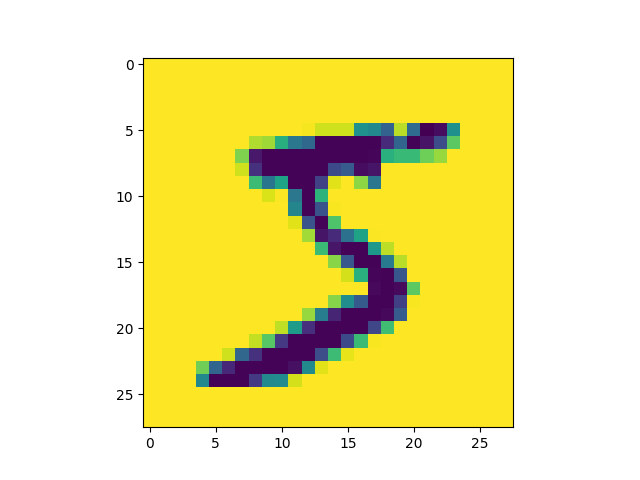
\includegraphics[width=0.6\textwidth]{img/5Raw.png}
    \caption{Obraz nieprzetworzony}
\end{figure}

\begin{figure}[H]
    \centering
    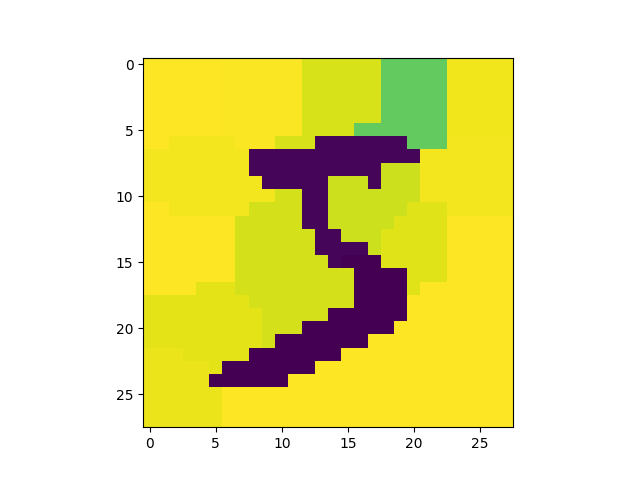
\includegraphics[width=0.6\textwidth]{img/5Sliced.png}
    \caption{Obraz z podziałem na superpiksele}
\end{figure}

\begin{figure}[H]
    \centering
    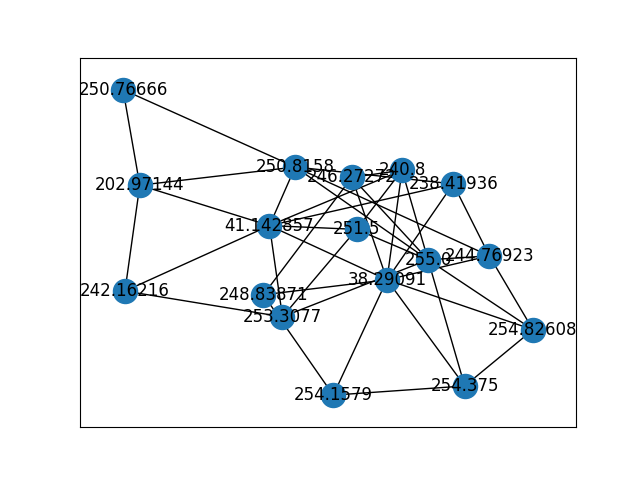
\includegraphics[width=0.6\textwidth]{img/5Graph.png}
    \caption{Graf powstały na bazie podzielonego obrazu.}
\end{figure}

Powyższe obrazy to wizualizacje macierzy zawierajacych jasności pikseli.
Oryginalne obrazy są czarno-białe.

Sieć grafowa została zbudowana w sposób następujący:
\begin{lstlisting}[style=siec]
    _________________________________________________________________
    Layer (type)                Output Shape              Param #
    =================================================================
    gcn_conv (GCNConv)          multiple                  100

    gcn_conv_1 (GCNConv)        multiple                  2550

    global_sum_pool (GlobalSumP  multiple                 0
    ool)

    dense (Dense)               multiple                  26112

    dense_1 (Dense)             multiple                  5130

    =================================================================
    Total params: 33,892
    Trainable params: 33,892
    Non-trainable params: 0
    _________________________________________________________________
\end{lstlisting}

\subsection{K Nearest Neighbours}
Model KNN został zaimplementowany z użyciem biblioteki numpy. Za parametr K 
wybrano wielokrotność liczności zbioru etykiet, 20.


\section{Wyniki}
\subsection{Drzewo decyzyjne}
Przykładowo dla następujących parametrów dla bazy MNIST-784:

\begin{itemize}
    \item max\_depth: 19
    \item max\_features: None
    \item min\_samples\_split: 5
    \item min\_samples\_leaf: 4
    \item criterion: entropy
    \item splitter: random
\end{itemize}
model osiągał skuteczność na danych testowych wynoszącą $0.873$.
\subsection{Las losowy}

Dla następujących parametrów dla bazy MNIST-784:

\begin{itemize}
    \item n\_estimators: 16
    \item max\_depth: 18
    \item max\_features: sqrt
    \item min\_samples\_split: 18
    \item min\_samples\_leaf: 1
    \item criterion: entropy
\end{itemize}
model osiągał skuteczność na danych testowych wynoszącą $0.951$.

\subsection{Własna implementacja Wielowarstwowego perceptronu}
Sieć wyuczono dla zbioru MNIST-784 i Fashion-MNIST. Dla MNIST-784 model trenowany był przez 50 epochów. Dla Fashion-MNIST przez 30 epochów.

\begin{figure}[H]
    \centering
    \includegraphics[width=0.6\textwidth]{../Saves/MyNetwork/mnist-784/MyNetwork_mnist_784_ep50_conf_mat.png}
    \caption{Macierz konfuzji modelu własnego MLP dla bazy MNIST-784 w zależności od epoki}
\end{figure}
Dla bazy MNIST-784 własna implementacja MLP osiągnęła accuracy równe $0.793$

\begin{figure}[H]
    \centering
    \includegraphics[width=0.6\textwidth]{../Saves/MyNetwork/mnist-784/MyNetwork_fashion-mnist_ep50_conf_mat.png}
    \caption{Macierz konfuzji modelu własnego MLP dla bazy MNIST-784 w zależności od epoki}
\end{figure}
Dla bazy Fashion-MNIST własna implementacja MLP osiągnęła accuracy równe $0.722$

\subsection{Wielowarstwowy perceptron Tensorflow Keras}

Sieć wyuczono dla dwóch zbiorów danych: MNIST-784 i Fashion-MNIST.
W obydwu przypadkach model był trenowany przez 500 epoch'ów.
Proces i rezultaty widoczne są na poniższych wykresach:

\subsubsection{MNIST-784}
\begin{figure}[H]
    \centering
    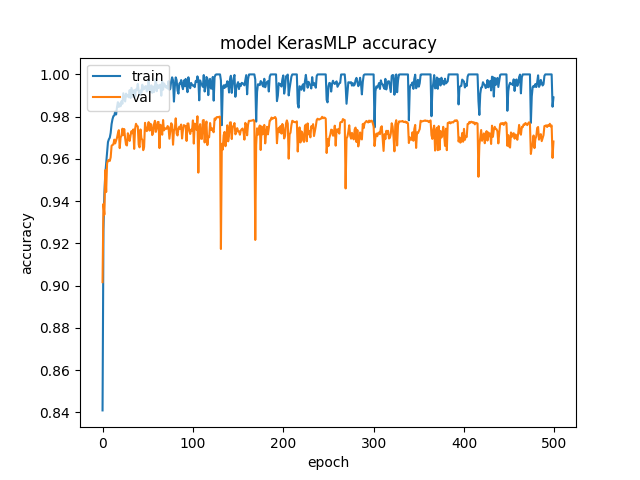
\includegraphics[width=0.6\textwidth]{../Saves/KerasMLP/mnist-784/KerasMLP_mnist_784_ep500_acc.png}
    \caption{Wykres dokładności modelu Keras MLP dla bazy MNIST-784 w zależności od epoki}
\end{figure}

\begin{figure}[H]
    \centering
    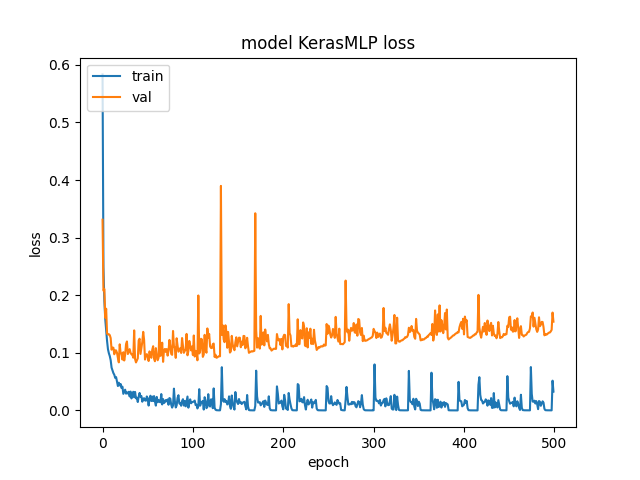
\includegraphics[width=0.6\textwidth]{../Saves/KerasMLP/mnist-784/KerasMLP_mnist_784_ep500_loss.png}
    \caption{Wykres wartości funkcji straty modelu Keras MLP dla bazy MNIST-784 w zależności od epoki} 
\end{figure}

\begin{figure}[H]
	\centering
	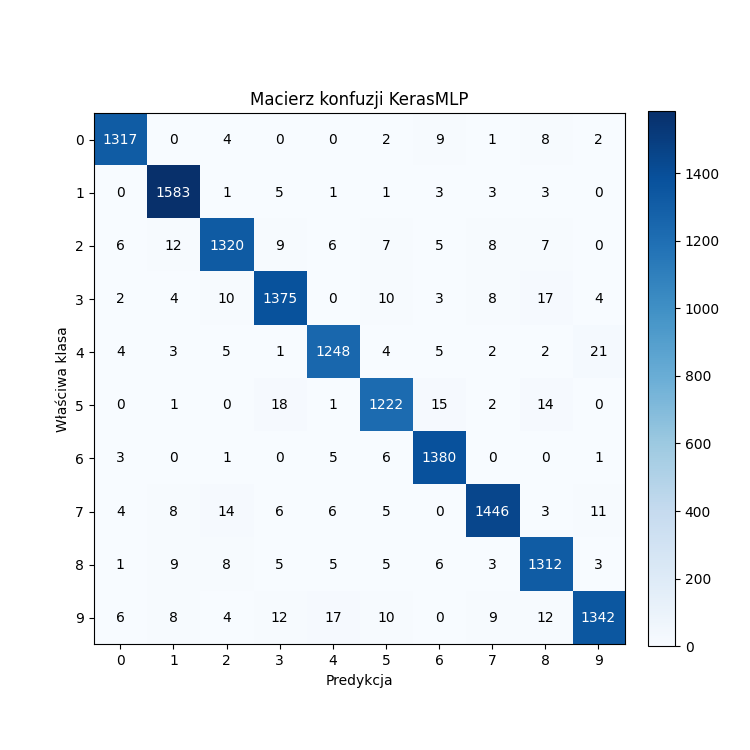
\includegraphics[width=0.6\textwidth]{../Saves/KerasMLP/mnist-784/KerasMLP_mnist_784_conf_mat.png}
	\caption{Macierz konfuzji modelu Keras MLP dla bazy MNIST-784}
\end{figure}
Dla bazy MNIST-784 model Keras MLP zdołał uzyskać accuracy w wysokości $0.975$

\subsubsection{Fashion-MNIST}
\begin{figure}[H]
    \centering
    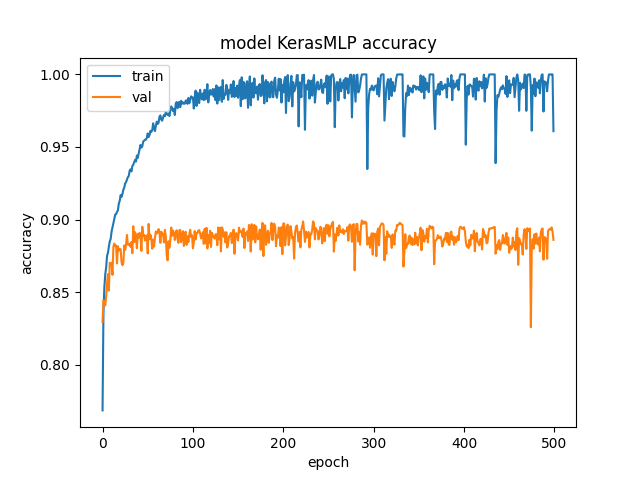
\includegraphics[width=0.6\textwidth]{../Saves/KerasMLP/fashion-mnist/KerasMLP_fashion-mnist_ep500_acc.png}
    \caption{Wykres dokładności modelu Keras MLP dla bazy Fashion-MNIST w zależności od epoki}
\end{figure}

\begin{figure}[H]
    \centering
    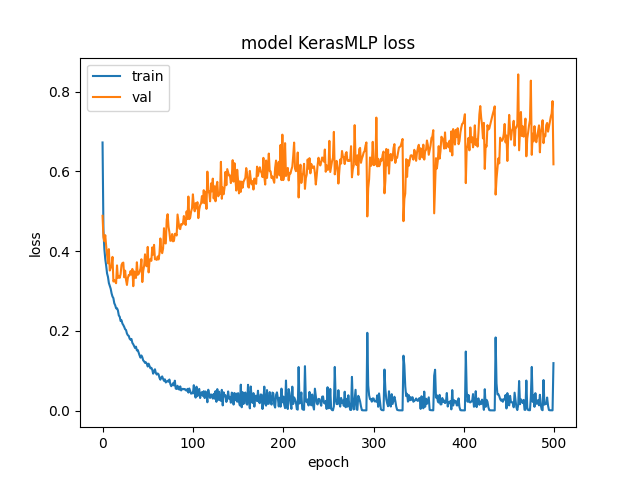
\includegraphics[width=0.6\textwidth]{../Saves/KerasMLP/fashion-mnist/KerasMLP_fashion-mnist_ep500_loss.png}
    \caption{Wykres wartości funkcji straty modelu Keras MLP dla bazy Fashion-MNIST w zależności od epoki}
\end{figure}

\begin{figure}[H]
	\centering
	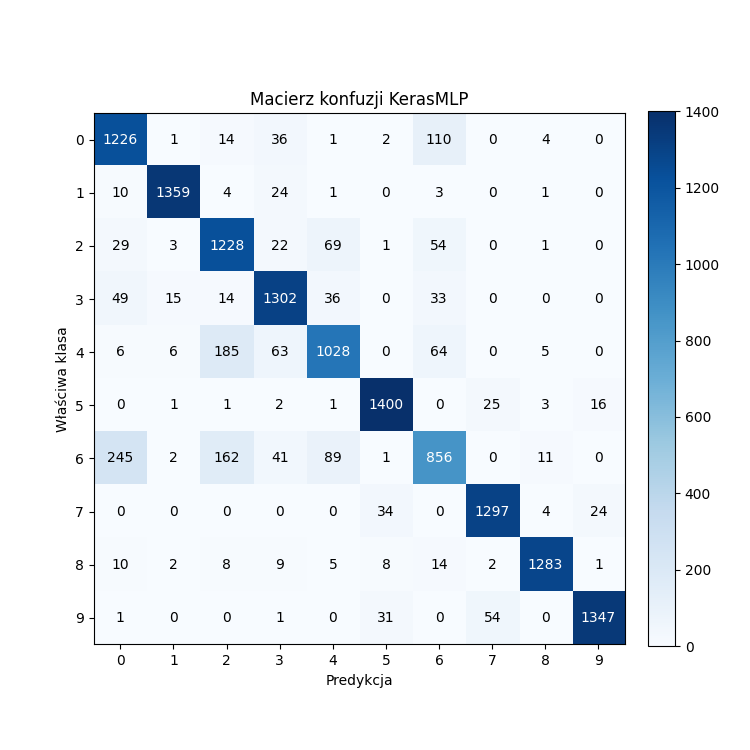
\includegraphics[width=0.6\textwidth]{../Saves/KerasMLP/fashion-mnist/KerasMLP_fashion-mnist_conf_mat.png}
	\caption{Macierz konfuzji modelu Keras MLP dla bazy Fashion-MNIST}
\end{figure}
Dla bazy Fashion-MNIST model Keras MLP zdołał uzyskać accuracy w wysokości $0.88$



\subsection{Sieć konwolucyjna Tensorflow Keras, wersja podstawowa}
Sieć wyuczono dla dwóch zbiorów danych: MNIST-784 i Fashion-MNIST. W obydwu przypadkach model
był trenowany przez 500 epoch'ów. Proces i rezultaty widoczne są na poniższych wykresach:

\subsubsection{MNIST-784}
\begin{figure}[H]
    \centering
    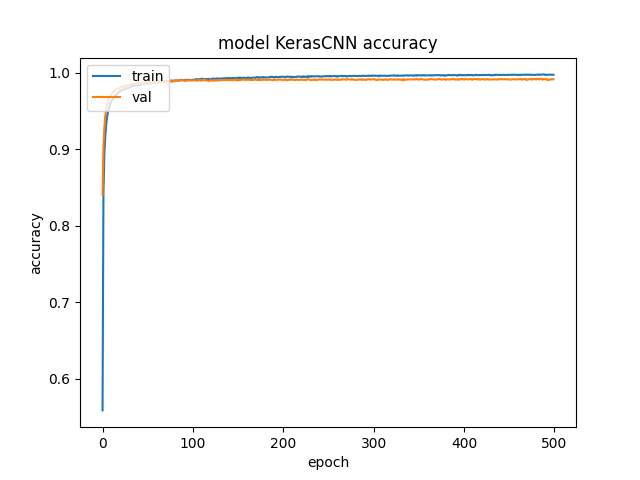
\includegraphics[width=0.6\textwidth]{../Saves/KerasCNN/mnist-784/KerasCNN_mnist_784_ep500_acc.png}
    \caption{Wykres dokładności modelu Keras CNN dla bazy MNIST-784 w zależności od epoki}
\end{figure}

\begin{figure}[H]
    \centering
    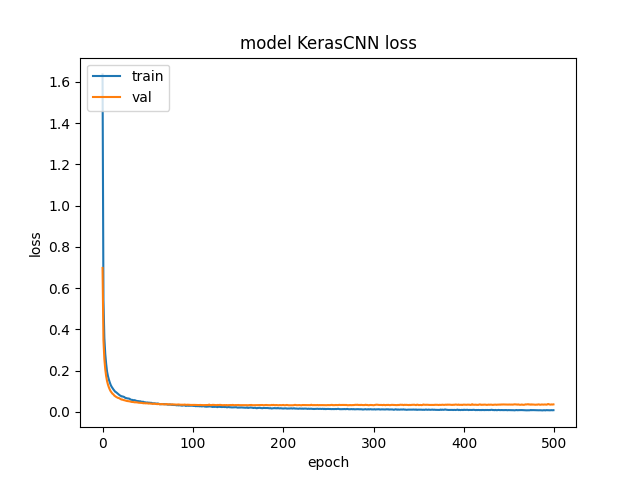
\includegraphics[width=0.6\textwidth]{../Saves/KerasCNN/mnist-784/KerasCNN_mnist_784_ep500_loss.png}
    \caption{Wykres wartości funkcji straty modelu Keras CNN dla bazy MNIST-784 w zależności od epoki} 
\end{figure}

\begin{figure}[H]
	\centering
	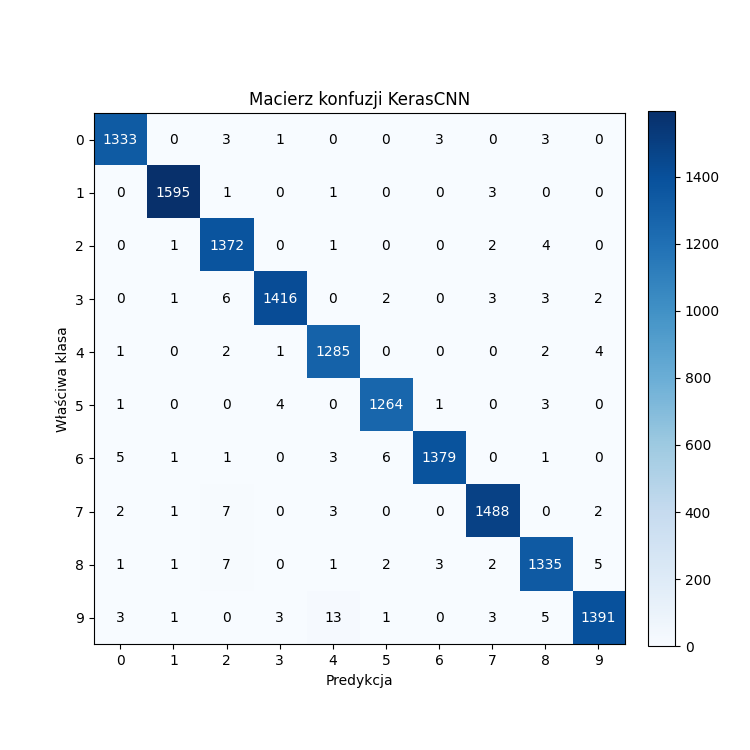
\includegraphics[width=0.6\textwidth]{../Saves/KerasCNN/mnist-784/KerasCNN_mnist_784_conf_mat.png}
	\caption{Macierz konfuzji modelu Keras CNN dla bazy MNIST-784}
\end{figure}
Dla bazy MNIST-784 model Keras CNN zdołał uzyskać accuracy w wysokości $0.9899$

\subsubsection{Fashion-MNIST}
\begin{figure}[H]
    \centering
    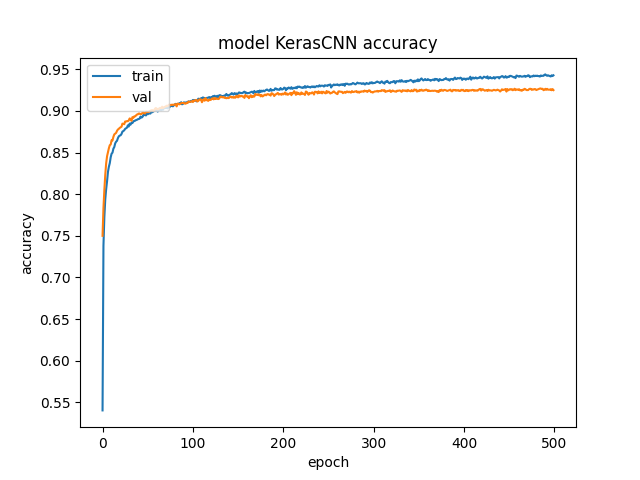
\includegraphics[width=0.6\textwidth]{../Saves/KerasCNN/fashion-mnist/KerasCNN_fashion-mnist_ep500_acc.png}
    \caption{Wykres dokładności modelu Keras CNN dla bazy Fashion-MNIST w zależności od epoki}
\end{figure}

\begin{figure}[H]
    \centering
    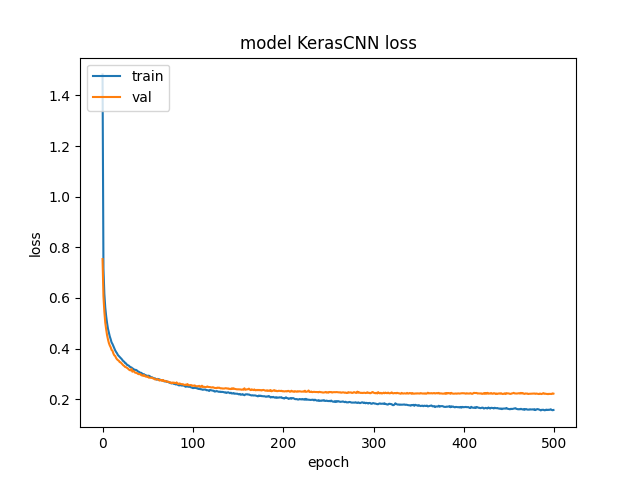
\includegraphics[width=0.6\textwidth]{../Saves/KerasCNN/fashion-mnist/KerasCNN_fashion-mnist_ep500_loss.png}
    \caption{Wykres wartości funkcji straty modelu Keras CNN dla bazy Fashion-MNIST w zależności od epoki}
\end{figure}

\begin{figure}[H]
	\centering
	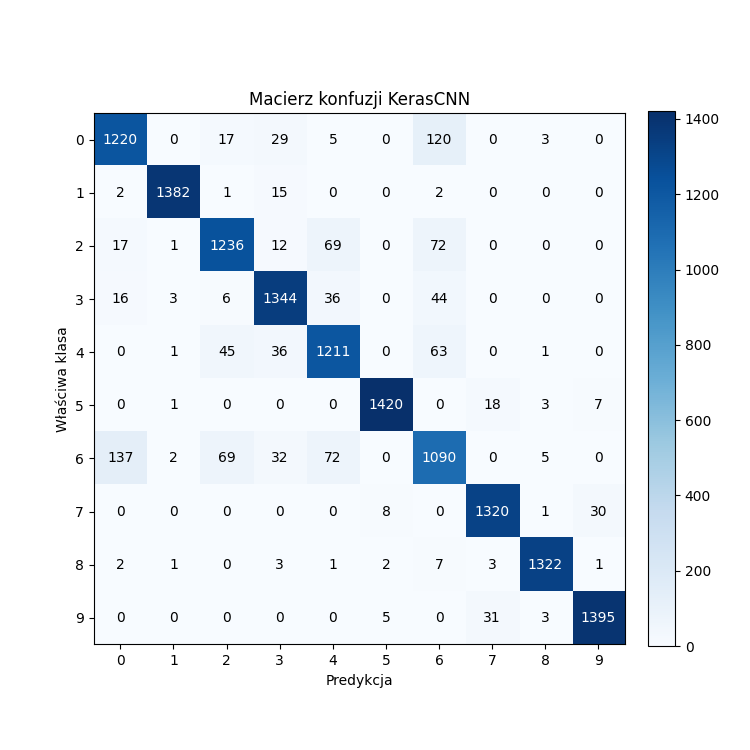
\includegraphics[width=0.6\textwidth]{../Saves/KerasCNN/fashion-mnist/KerasCNN_fashion-mnist_conf_mat.png}
	\caption{Macierz konfuzji modelu Keras CNN dla bazy Fashion-MNIST}
\end{figure}
Dla bazy Fashion-MNIST model Keras CNN zdołał uzyskać accuracy w wysokości $0.924$


\subsection{Sieć konwolucyjna Tensorflow Keras, wersja rozszerzona}
Sieć wyuczono dla dwóch zbiorów danych: MNIST-784 i Fashion-MNIST. Dzięki zastosowaniu callbacków proces trenowania w przypadku bazy MNIST-784 trwał 32 epochy a w przypadku Fashion-MNIST 47 epochów. Proces i rezultaty widoczne są na poniższych wykresach:

\subsubsection{MNIST-784}
\begin{figure}[H]
    \centering
    \includegraphics[width=0.6\textwidth]{../Saves/KerasCNNV2/mnist-784/KerasCNNV2_mnist_784_ep32_acc.png}
    \caption{Wykres dokładności modelu Keras CNN dla bazy MNIST-784 w zależności od epoki}
\end{figure}

\begin{figure}[H]
    \centering
    \includegraphics[width=0.6\textwidth]{../Saves/KerasCNNV2/mnist-784/KerasCNNV2_mnist_784_ep32_loss.png}
    \caption{Wykres wartości funkcji straty modelu Keras CNNv2 dla bazy MNIST-784 w zależności od epoki} 
\end{figure}

\begin{figure}[H]
	\centering
	\includegraphics[width=0.6\textwidth]{../Saves/KerasCNNV2/mnist-784/KerasCNNV2_mnist_784_conf_mat.png}
	\caption{Macierz konfuzji modelu Keras CNNv2 dla bazy MNIST-784}
\end{figure}
Dla bazy MNIST-784 model Keras CNNv2 zdołał uzyskać accuracy w wysokości $0.9924$

\subsubsection{Fashion-MNIST}
\begin{figure}[H]
    \centering
    \includegraphics[width=0.6\textwidth]{../Saves/KerasCNNV2/fashion-mnist/KerasCNNV2_fashion-mnist_ep47_acc.png}
    \caption{Wykres dokładności modelu Keras CNN dla bazy Fashion-MNIST w zależności od epoki}
\end{figure}

\begin{figure}[H]
    \centering
    \includegraphics[width=0.6\textwidth]{../Saves/KerasCNNV2/fashion-mnist/KerasCNNV2_fashion-mnist_ep47_loss.png}
    \caption{Wykres wartości funkcji straty modelu Keras CNNv2 dla bazy Fashion-MNIST w zależności od epoki}
\end{figure}

\begin{figure}[H]
	\centering
	\includegraphics[width=0.6\textwidth]{../Saves/KerasCNNV2/fashion-mnist/KerasCNNV2_fashion-mnist_conf_mat.png}
	\caption{Macierz konfuzji modelu Keras CNNv2 dla bazy Fashion-MNIST}
\end{figure}
Dla bazy Fashion-MNIST model Keras CNNv2 zdołał uzyskać accuracy w wysokości $0.912$


\subsection{Sieć transferowa Tensorflow Keras}
Sieć wyuczono dla dwóch zbiorów danych: MNIST-784 i Fashion-MNIST. W obydwu
przypadkach model trenowany był najpierw przez 10 epochów, następnie
przez 100 epochów z fine tuningiem. Proces i rezultaty widoczne są na poniższych wykresach:

\subsubsection{MNIST-784}
\begin{figure}[H]
    \centering
    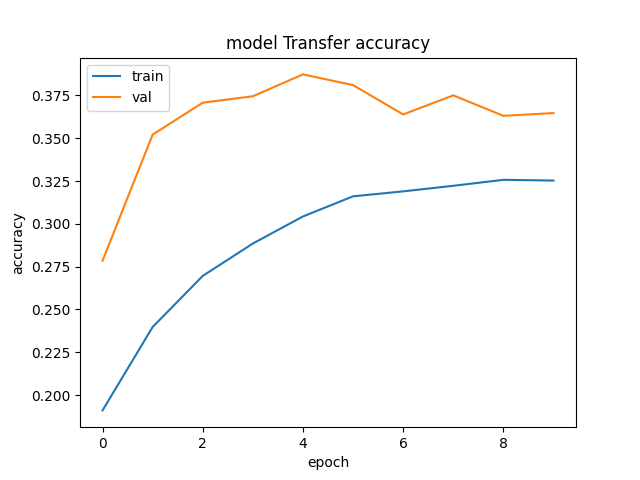
\includegraphics[width=0.6\textwidth]{../Saves/Transfer/mnist-784/Transfer_mnist_784_ep10_acc.png}
    \caption{Wykres dokładności modelu Transferowego dla bazy MNIST-784 w zależności od epoki w trenowaniu wstępnym}
\end{figure}

\begin{figure}[H]
    \centering
    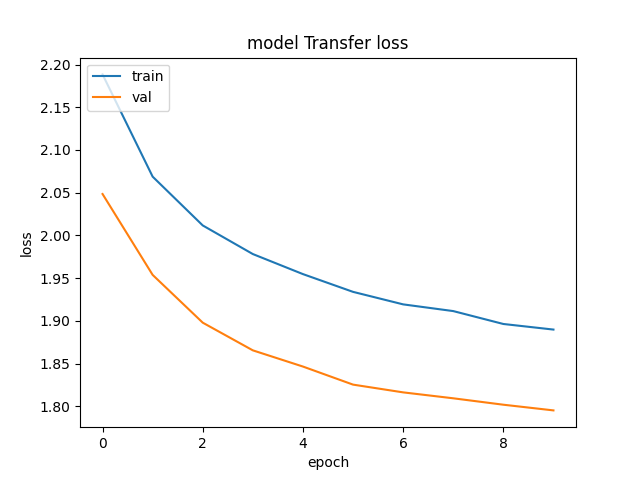
\includegraphics[width=0.6\textwidth]{../Saves/Transfer/mnist-784/Transfer_mnist_784_ep10_loss.png}
    \caption{Wykres wartości funkcji straty modelu Transferowego dla bazy MNIST-784 w zależności od epoki w trenowaniu wstępnym} 
\end{figure}

\begin{figure}[H]
    \centering
    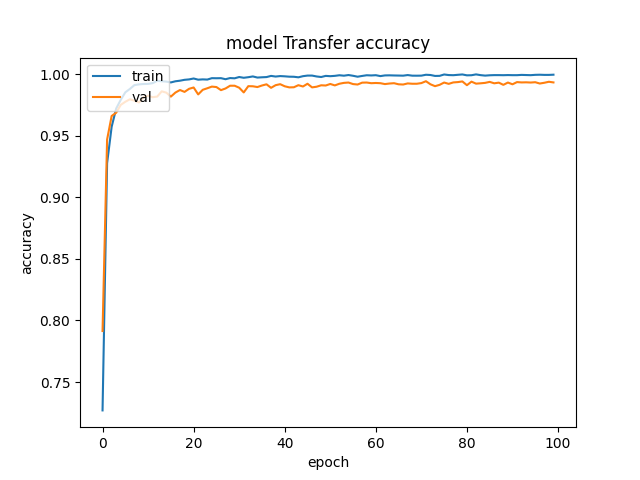
\includegraphics[width=0.6\textwidth]{../Saves/Transfer/mnist-784/Transfer_mnist_784_ep100_acc.png}
    \caption{Wykres dokładności modelu Transferowego dla bazy MNIST-784 w zależności od epoki w fine tuningu}
\end{figure}

\begin{figure}[H]
    \centering
    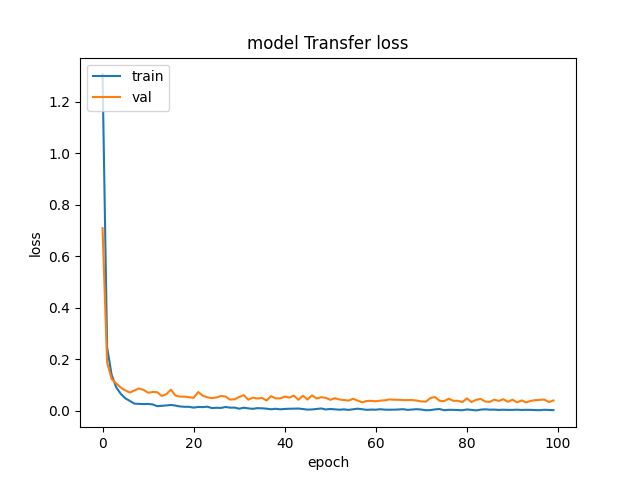
\includegraphics[width=0.6\textwidth]{../Saves/Transfer/mnist-784/Transfer_mnist_784_ep100_loss.png}
    \caption{Wykres wartości funkcji straty modelu Transferowego dla bazy MNIST-784 w zależności od epoki w fine tuningu} 
\end{figure}

\begin{figure}[H]
	\centering
	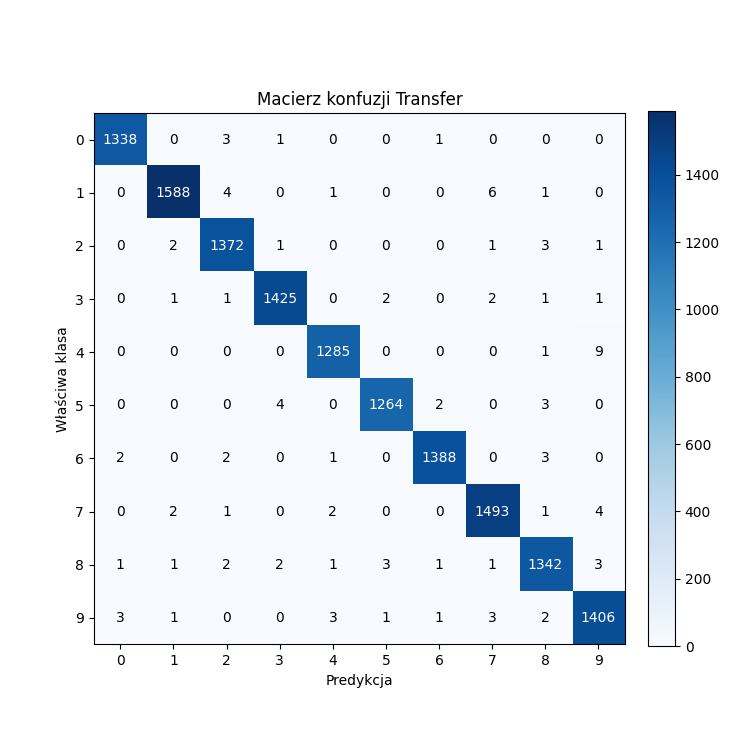
\includegraphics[width=0.6\textwidth]{../Saves/Transfer/mnist-784/Transfer_mnist_784_conf_mat.png}
	\caption{Macierz konfuzji modelu Transferowego dla bazy MNIST-784}
\end{figure}
Dla bazy MNIST-784 model Keras CNN zdołał uzyskać accuracy w wysokości $0.9929$

\subsubsection{Fashion-MNIST}
\begin{figure}[H]
    \centering
    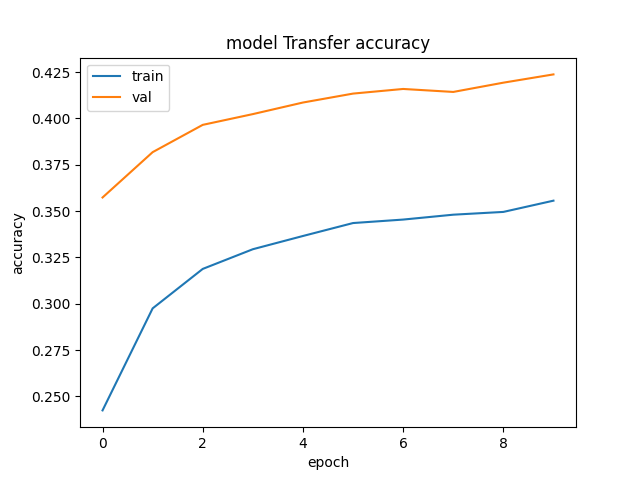
\includegraphics[width=0.6\textwidth]{../Saves/Transfer/fashion-mnist/Transfer_fashion-mnist_ep10_acc.png}
    \caption{Wykres dokładności modelu Transferowego dla bazy Fashion-MNIST w zależności od epoki w trenowaniu wstępnym}
\end{figure}

\begin{figure}[H]
    \centering
    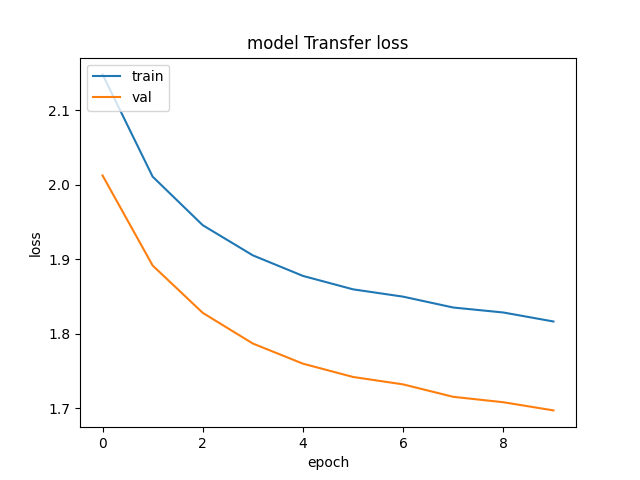
\includegraphics[width=0.6\textwidth]{../Saves/Transfer/fashion-mnist/Transfer_fashion-mnist_ep10_loss.png}
    \caption{Wykres wartości funkcji straty modelu Transferowego dla bazy Fashion-MNIST w zależności od epoki w trenowaniu wstępnym}
\end{figure}

\begin{figure}[H]
    \centering
    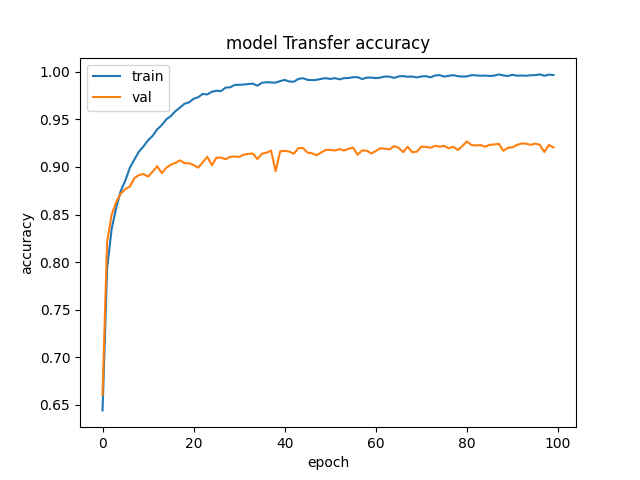
\includegraphics[width=0.6\textwidth]{../Saves/Transfer/fashion-mnist/Transfer_fashion-mnist_ep100_acc.png}
    \caption{Wykres dokładności modelu Transferowego dla bazy Fashion-MNIST w zależności od epoki w fine tuningu}
\end{figure}

\begin{figure}[H]
    \centering
    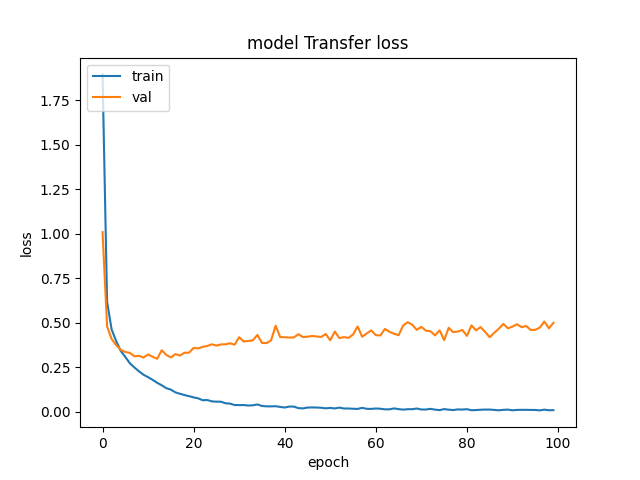
\includegraphics[width=0.6\textwidth]{../Saves/Transfer/fashion-mnist/Transfer_fashion-mnist_ep100_loss.png}
    \caption{Wykres wartości funkcji straty modelu Transferowego dla bazy Fashion-MNIST w zależności od epoki w fine tuningu} 
\end{figure}

\begin{figure}[H]
	\centering
	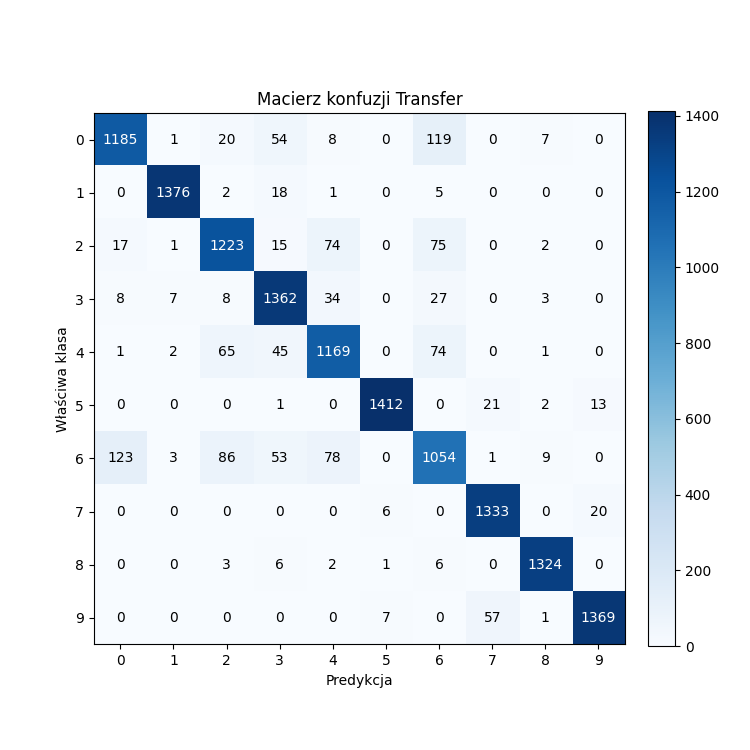
\includegraphics[width=0.6\textwidth]{../Saves/Transfer/fashion-mnist/Transfer_fashion-mnist_conf_mat.png}
	\caption{Macierz konfuzji modelu Transferowego dla bazy Fashion-MNIST}
\end{figure}
Dla bazy Fashion-MNIST model Keras CNN zdołał uzyskać accuracy w wysokości $0.9148$

\subsection{Sieć grafowa}

\subsubsection{Zbiór A}

Wyniki dla zbioru A:
\begin{itemize}
    \item Loss: 1.9428
    \item Accuracy: 0.2689
\end{itemize}

\begin{figure}[H]
    \centering
    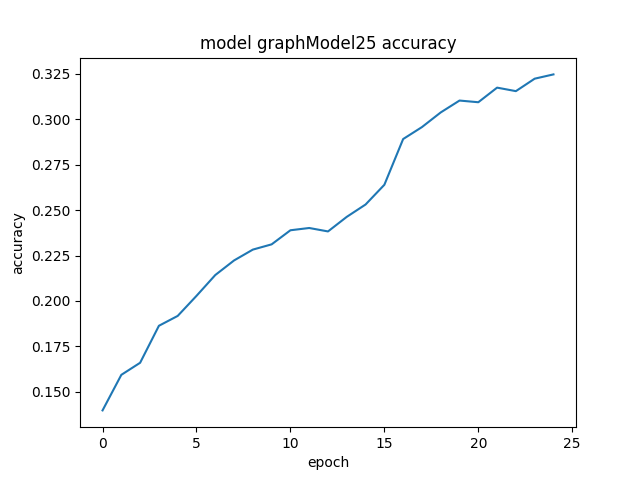
\includegraphics[width=0.6\textwidth]{img/graphModel25_acc.png}
    \caption{Wykres celności dla modelu grafowego trenowanego na zbiorze A w zależności od epoki}
\end{figure}

\begin{figure}[H]
    \centering
    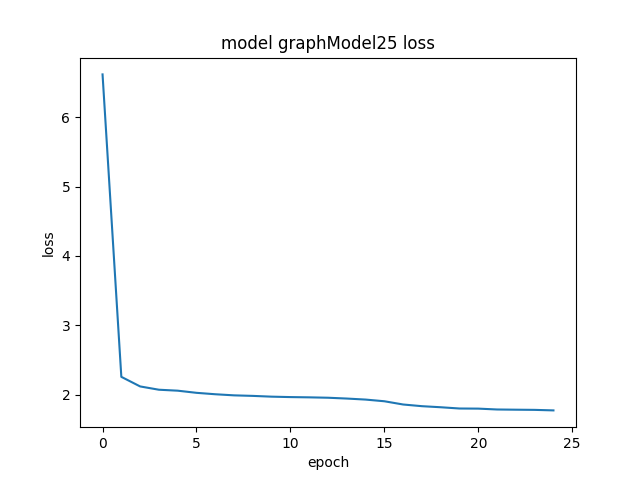
\includegraphics[width=0.6\textwidth]{img/graphModel25_loss.png}
    \caption{Wykres wartości funkcji straty dla modelu grafowego trenowanego na zbiorze A w zależności od epoki}
\end{figure}

\begin{figure}[H]
    \centering
    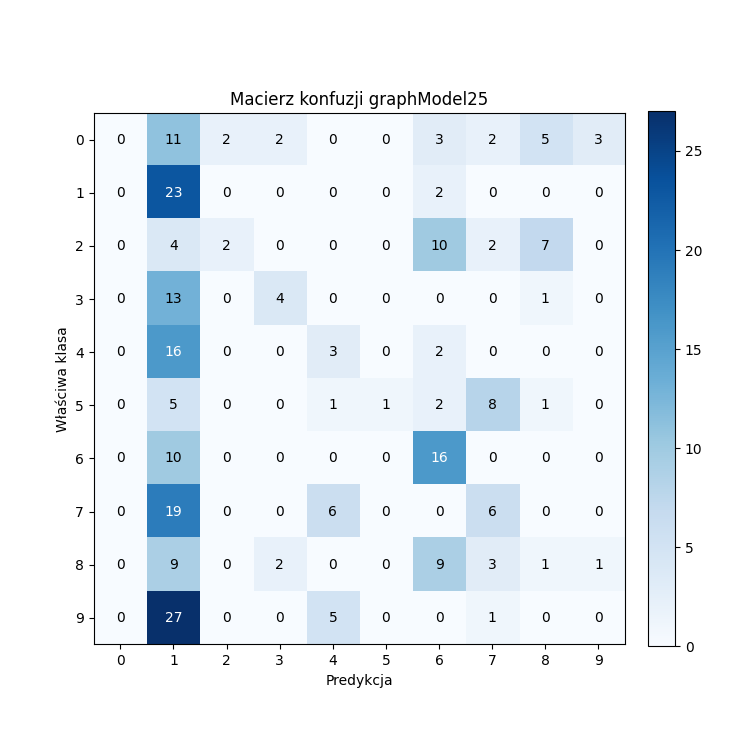
\includegraphics[width=0.6\textwidth]{img/graphModel25_confusion.png}
    \caption{Macierz konfuzji dla modelu grafowego trenowanego na zbiorze A w zależności od epoki}
\end{figure}

\subsubsection{Zbiór B}

Wyniki dla zbioru B:
\begin{itemize}
    \item Loss: 2.7640
    \item Accuracy: 0.1205
\end{itemize}

\begin{figure}[H]
    \centering
    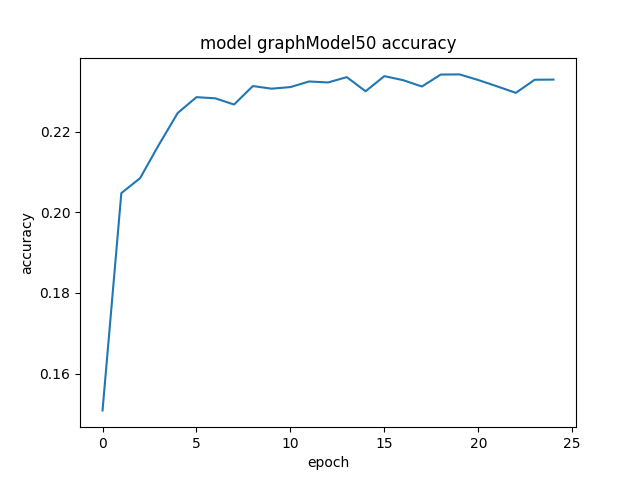
\includegraphics[width=0.6\textwidth]{img/graphModel50_acc.png}
    \caption{Wykres celności dla modelu grafowego trenowanego na zbiorze B w zależności od epoki}
\end{figure}

\begin{figure}[H]
    \centering
    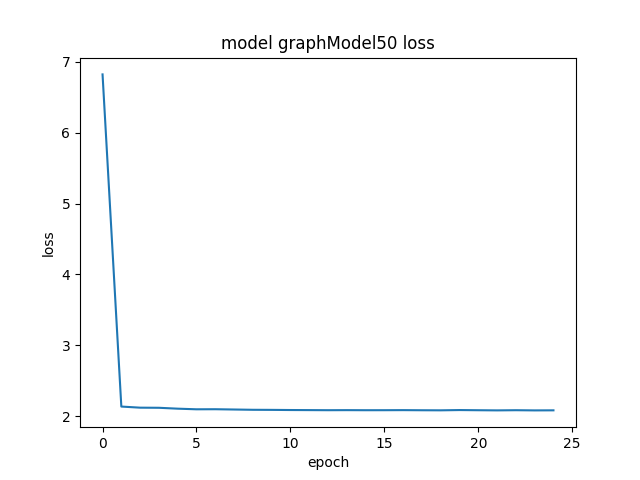
\includegraphics[width=0.6\textwidth]{img/graphModel50_loss.png}
    \caption{Wykres wartości funkcji straty dla modelu grafowego trenowanego na zbiorze B w zależności od epoki}
\end{figure}

\begin{figure}[H]
    \centering
    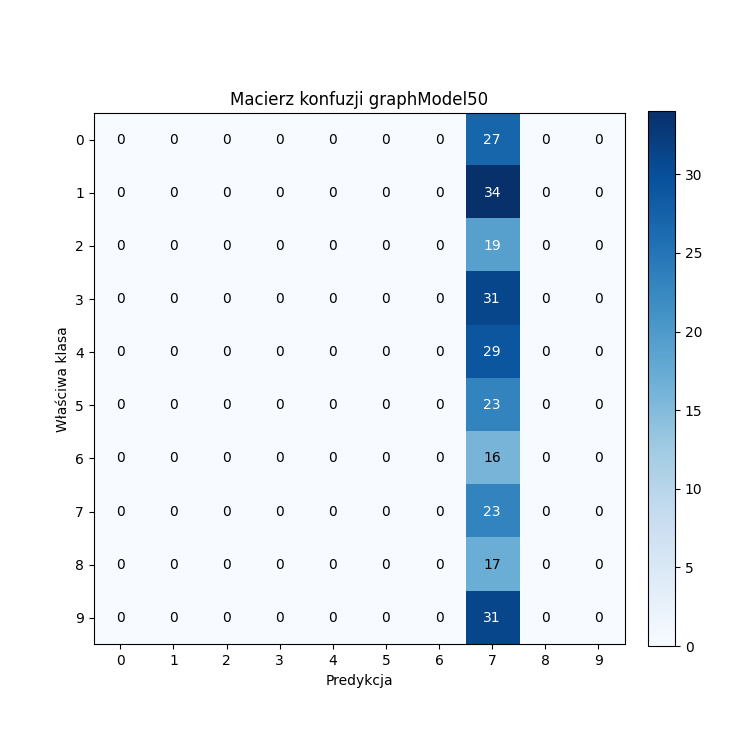
\includegraphics[width=0.6\textwidth]{img/graphModel50_confusion.png}
    \caption{Macierz konfuzji dla modelu grafowego trenowanego na zbiorze B w zależności od epoki}
\end{figure}

\subsubsection{Zbiór C}

Wyniki dla zbioru C:
\begin{itemize}
    \item Loss: 3.5503
    \item Accuracy: 0.0924
\end{itemize}

\begin{figure}[H]
    \centering
    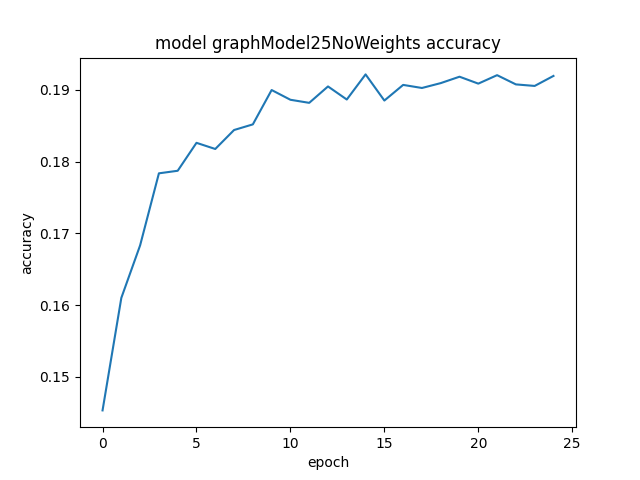
\includegraphics[width=0.6\textwidth]{img/graphModel25NoWeights_acc.png}
    \caption{Wykres celności dla modelu grafowego trenowanego na zbiorze C w zależności od epoki}
\end{figure}

\begin{figure}[H]
    \centering
    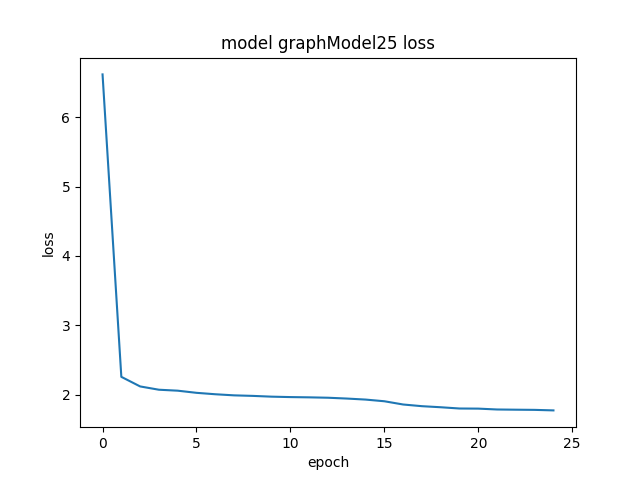
\includegraphics[width=0.6\textwidth]{img/graphModel25_loss.png}
    \caption{Wykres wartości funkcji straty dla modelu grafowego trenowanego na zbiorze C w zależności od epoki}
\end{figure}

\begin{figure}[H]
    \centering
    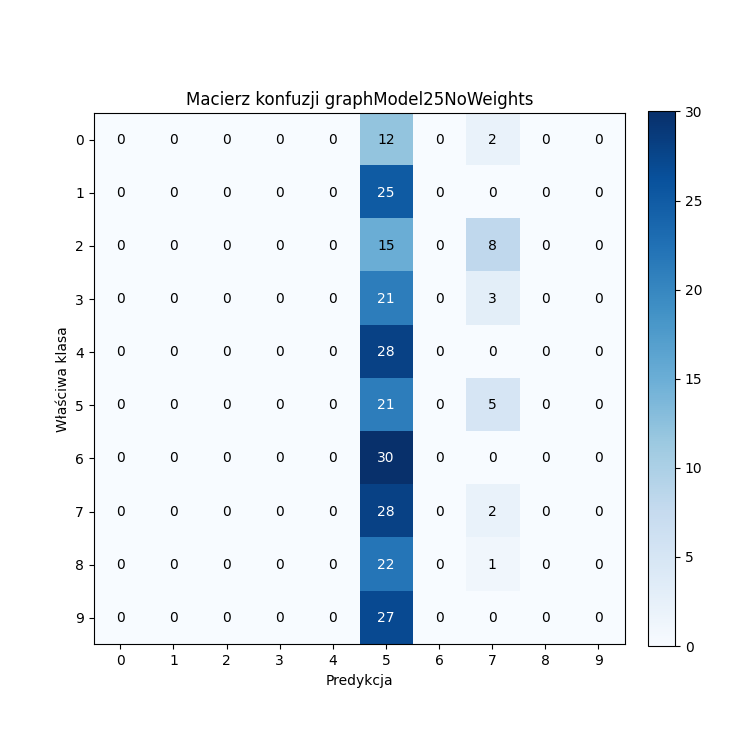
\includegraphics[width=0.6\textwidth]{img/graphModel25NoWeights_confusion.png}
    \caption{Macierz konfuzji dla modelu grafowego trenowanego na zbiorze C w zależności od epoki}
\end{figure}

Sieć w żadnym z przypadków nie uzyskała zbyt imponujących
wyników: celność w najlepszym wypadku wynosiła około 25\%.

Można zauważyć, że zwiększanie ilości danych nie musi
prowadzić do poprawienia wyników: w przypadku bardziej
szczegółowych grafów o max. 50 wierzchołkach, wyniki były
dużo słabsze niż w prostszym przypadku, gdzie grafy nie
miały więcej niż 25 wierzchołków.

O ile redukcja liczby wierzchołków ułatwiała sieci zadanie,
to już usunięcie informacji o wagach krawędzi sprawiło,
że zaczęła ona uzyskiwać fatalne wyniki.

W oczy rzuca się także fakt, że badany model grafowy ma
wyraźną tendencję do faworyzowania jednej konkretnej klasy
i przypisywania do niej większości grafów - to zjawisko jest
wyraźnie widoczne nawet w najlepszym spośród badanych przypadków.

\subsection{K Nearest Neighbours}
Model KNN przetestowano dla bazy danych MNIST i Fashion-MNIST.

Z powodu bardzo długiego czasu predykcji modelu KNN testy wykonano na 10\% zbioru testowego, co odpowiada 1400 danych testowych.
Z powodu długiego czasu predykcji modelu KNN testy wykonano na 10\% zbioru
testowego, co odpowiada 1400 danych testowych.

Dla bazy MNIST-784 model KNN osiągnął accuracy równe $0.96$

Dla bazy Fashion-MNIST model KNN osiągnął accuracy równe $0.86$


\section{Dyskusja}

Lorem ipsum dolor sit amet, consectetur adipiscing elit.
Sed vitae quam euismod, aliquam elit quis, ultricies nisl.
Sed euismod, nisl quis aliquam ultricies, nisl nisl aliquam elit,
quis aliquam elit nisl quis aliquam elit nisl quis aliquam elit.
Sed euismod, nisl quis aliquam elit nisl quis aliquam elit.
Sed euismod, nisl quis aliquam elit nisl quis aliquam elit.
Sed euismod, nisl quis aliquam elit nisl quis aliquam elit.
Sed euismod, nisl quis aliquam elit nisl quis aliquam elit.

\renewcommand{\refname}{Źródła}
\begin{thebibliography}{100}
    % \bibitem{bib:1} Autor,
    % \textit{tytuł}, 2022
    % \\\url{https://www.example.com}
\end{thebibliography}

\end{document}


